\documentclass{ctexart}
\usepackage{amsmath,bm}
\usepackage{setspace}
\usepackage{xeCJK}
\usepackage{xcolor}
\usepackage{indentfirst}
\usepackage{listings}
\usepackage{graphicx}
\usepackage{subfigure}
\usepackage{amsfonts,amssymb}
\usepackage[a4paper,scale=0.8]{geometry}
\usepackage{hyperref}
\usepackage{float}
\usepackage{listings}
\usepackage{changepage}
\lstset{language=verilog}%这条命令可以让LaTeX排版时将C++键字突出显示

\lstset{breaklines}%这条命令可以让LaTeX自动将长的代码行换行排版

\lstset{extendedchars=false}%这一条命令可以解决代码跨页时,章节标题,页眉等汉字不显示的问题
\setCJKmainfont{华光书宋_CNKI}
\newCJKfontfamily\kaiti{华光楷体_CNKI}
\newCJKfontfamily\hei{华光黑体_CNKI}
\newCJKfontfamily\fsong{华光仿宋_CNKI}
\newfontfamily\code{Courier New}
\linespread{1.5} \setlength\parindent{2 em}
\title{\Huge 中国科学技术大学计算机学院\\《计算机体系结构》实验报告}
\date{\LARGE 2021.06.10}
\begin{document}
\begin{hei}  \maketitle\end{hei}
\begin{figure}[htbp]
    \centering
    
\includegraphics[scale=0.4]{USTC.png}

\end{figure}
\begin{LARGE}\begin{align*}  & \text{实验题目:\underline{分支预测}}   \\
         & \text{学生姓名:\underline{胡毅翔}}     \\
         & \text{学生学号:\underline{PB18000290}}\end{align*}\end{LARGE}
\par
\par\par
\centerline{\large 计算机实验教学中心制}
\par \centerline {\large 2019年9月}
\newpage
\section{\hei 实验目的}
\begin{enumerate}
    \item 实现BTB(Branch Target Buffer)和BHT(Branch History Table)两种动态分支预测器。
    \item 体会动态分支预测对流水线性能的影响。

\end{enumerate}
\section{\hei 实验环境}
\begin{enumerate}
    \item PC一台
    \item Windows 10操作系统
    \item Vivado 2019.1
    \item Visual Studio Code 1.56.2
\end{enumerate}

\section{\hei BTB实现}
BTB(Branch Target Buffer)是动态分支预测的一种基本方法。它使用一个Buffer,里面记录了历史指令跳转信息。对于每一条跳转的Branch指令,它都将其写入buffer,记录其跳转的地址,并有一个标志位标记最近一次执行是否跳转。这样如果有一条在Buffer里的跳转指令将执行时,可以根据buffer记录的历史跳转信息,预测下一条要执行的指令地址,预测正确的话可以减小分支开销。BTB只使用了1-bit的历史信息,也可以视作1-bit BHT。
\par

在我们之前实现的lab2 RV32I Core中,下一条PC地址是PC + 4。在添加了BTB之后,对于IF阶段产生的PC,在BTB Buffer里检查是否有对应项,如果有的话,根据其历史跳转记录,确定是否选择predicted PC作为下一PC。如果当前PC不在BTB表里,但在EX段发现是一条需要跳转的Branch指令,则在EX阶段更新BTB表。另外,如果PC在BTB表中,在EX阶段发现预测的跳转失败,也需要更新BTB表,并flush错误装载的指令。
\par
主要设计参照如下图所示,其中Branch PC标记对应程序中的BranchTagAddress变量, Predicted PC对应存储的预测结果对应程序中的BranchTargetAddress变量。
当IF阶段产生的指令在BTB表中找到对应的一项并且最近一次跳转的标志位为真,则将预测结果有效变量改为1,将预测的PC值从BTB表中取出。
当EX阶段的操作码表示当前指令是BR类指令时。当EX阶段的PC值在BTB表中有存储时,更新PC值对应的预测PC值为br\_target值,并将是否跳转的标示量更改
为br对应的值;如果不存在对应的存储,则按照FIFO顺序进行BTB表的写入。\par
\begin{figure}[H]
    \centering
    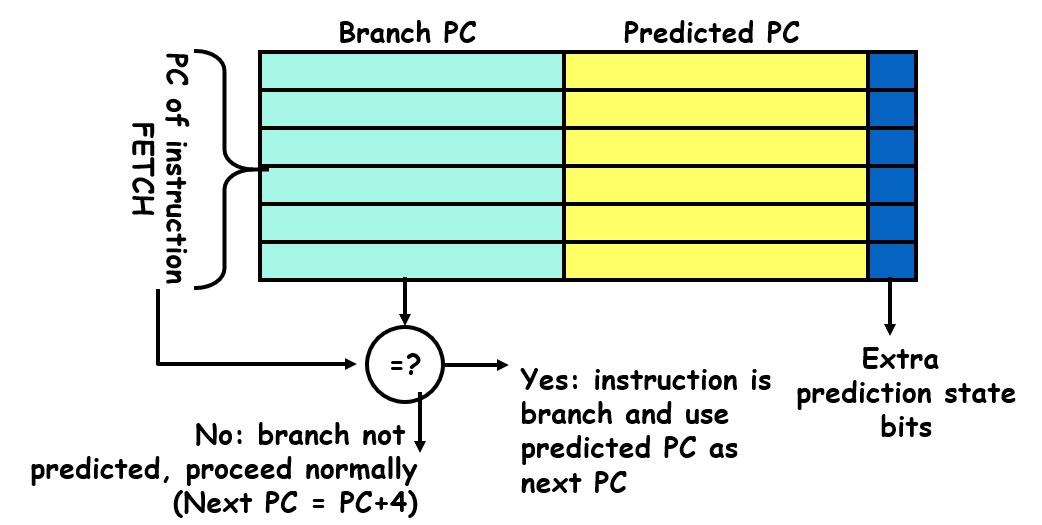
\includegraphics[scale=0.45]{btb.png}
    \caption{BTB}
\end{figure}
状态机如下图。
\par

\begin{figure}[H]
    \centering
    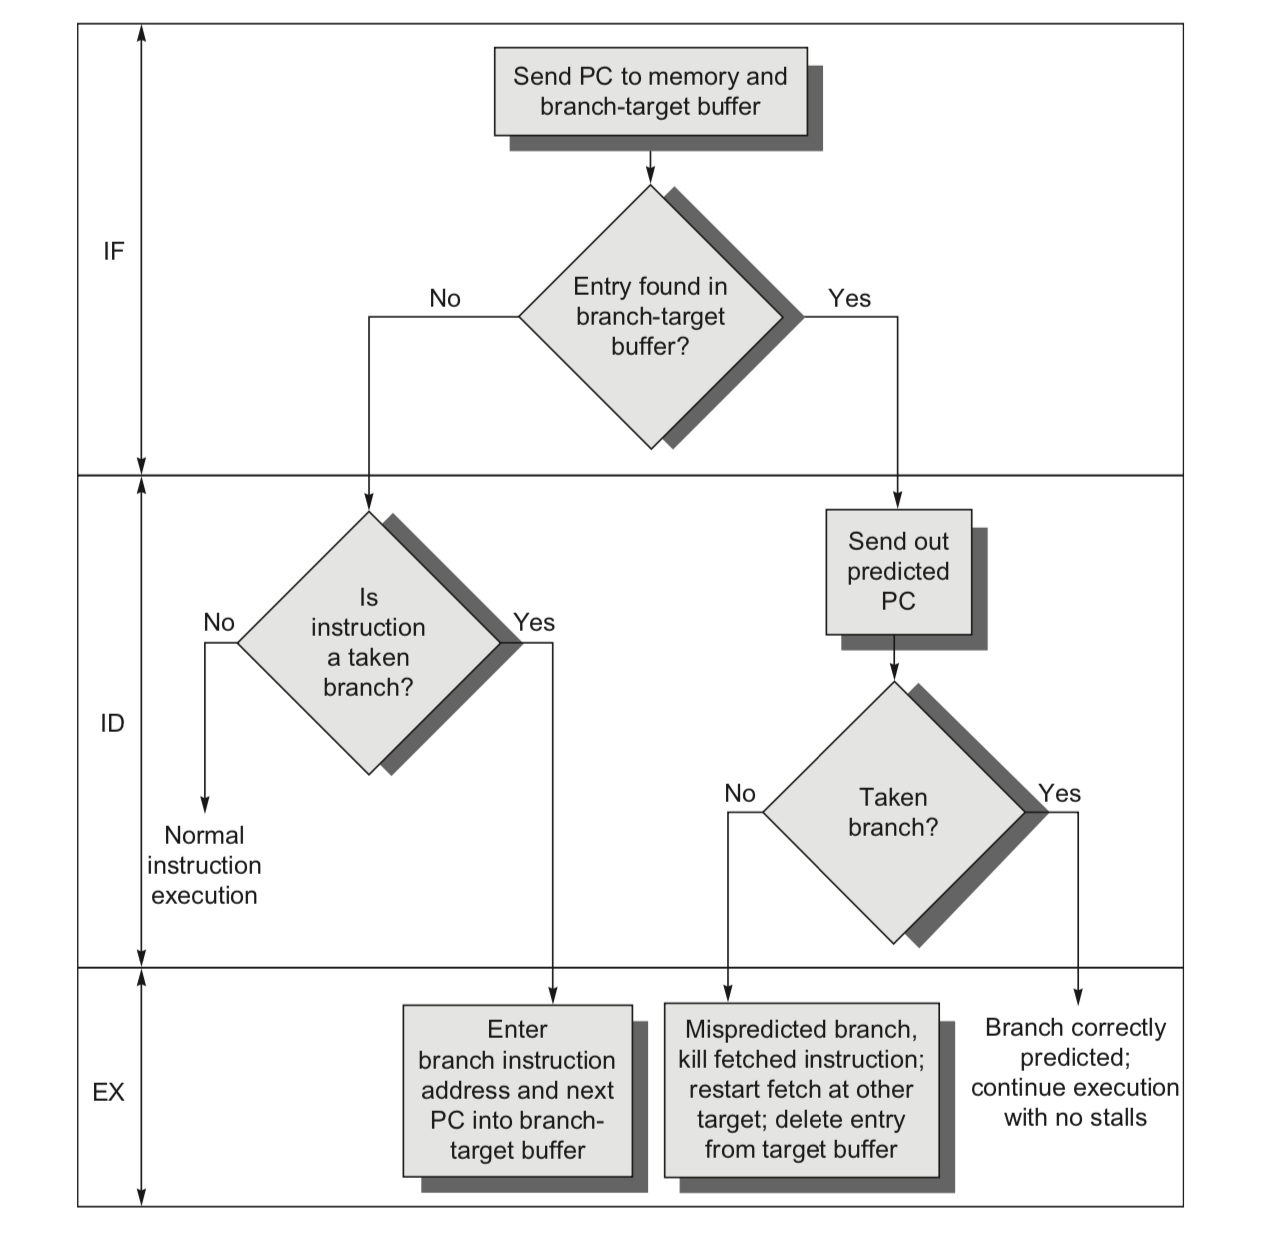
\includegraphics[scale=0.45]{ztj.png}
    \caption{BTB状态机}
\end{figure}


\par 实现的代码如下:
\begin{lstlisting}
module btb # (
    parameter ENTRY_NUM = 64//BTB大小
)(
    input clk, 
    input rst, 
    input [31:0] PC_IF, 
    input [31:0] PC_EX, 
    input [31:0] br_target, 
    input br, 
    input [6:0] Opcode_EX, 
    output reg [31:0] PredictPC, //PC预测结果
    output reg PredictPCValid      //预测结果有效
);
//分支Opcode
localparam BR_OP = 7'b110_0011; 
//Buffer define
reg [31:0] BranchTagAddress[ENTRY_NUM - 1 : 0]; 
reg [31:0] BranchTargetAddress[ENTRY_NUM - 1 : 0]; 
reg Valid[ENTRY_NUM - 1 : 0]; 
//FIFO Index
reg [15 : 0] Index; 
//Produce PredictPC
always @ (*) begin
    if (rst) begin
        PredictPC <= 32'b0; 
        PredictPCValid <= 1'b0; 
    end
    else begin
        PredictPC <= 32'b0; 
        PredictPCValid <= 1'b0; 
        for (integer i = 0; i < ENTRY_NUM ; i++ ) begin
            if ((PC_IF == BranchTagAddress[i]) && Valid[i]) begin
                PredictPCValid <= 1'b1; 
                PredictPC <= BranchTargetAddress[i]; 
            end
        end
    end
end 
//Renew Buffer
always @ (posedge clk or posedge rst) begin
    if (rst) begin
        for (integer i = 0; i < ENTRY_NUM ; i++ ) begin
            Valid[i] <= 1'b0; 
            BranchTagAddress[i] <= 32'd0; 
            BranchTargetAddress[i] <= 32'd0; 
        end
        Index <= 16'd0; 
    end
    else begin
        if (Opcode_EX == BR_OP) begin
            integer i; 
            for (i = 0; i < ENTRY_NUM; i++) begin
                if (PC_EX == BranchTagAddress[i]) begin
                    BranchTargetAddress[i] <= br_target; 
                    Valid[i] <= br; 
                    break; 
                end
            end
            if (i == ENTRY_NUM) begin
                BranchTargetAddress[Index] <= br_target; 
                Valid[Index] <= br; 
                BranchTagAddress[Index] <= PC_EX; 
                Index = Index + 1; 
            end
        end
    end
end
endmodule
\end{lstlisting}
\section{\hei BHT实现}
BHT(Branch History Table)是动态分支预测的另一种基本策略。类似BTB,它也维护了一个N * 2的cache作为buffer。其中,N是BHT表的项数(一般取4096项),根据PC的低位查找BHT表,每个项都维护了一个独立的2-bit状态机。如下图:
\begin{figure}[H]
    \centering
    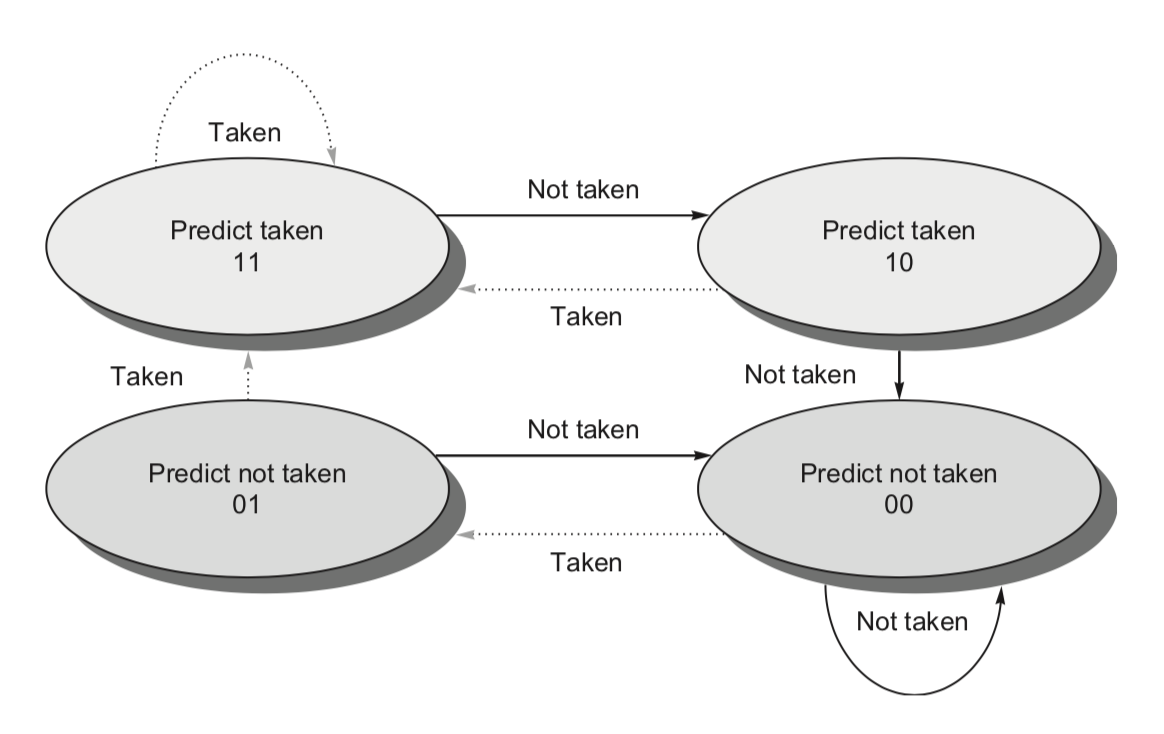
\includegraphics[scale=0.45]{bhtztj.png}
    \caption{BHT状态机}
\end{figure}
\par
BHT和BTB一样,在IF阶段对当前PC预测其是否跳转。相较于BTB,BHT的预测准确度更高,在IF阶段,首先判断当前PC在BTB表中是否跳转,如果跳转,再到BHT表中寻找其是否跳转。只有两者都预测跳转时,才预测当前指令跳转,并将BTB表中的预测跳转地址作为下一条指令的PC地址。特别的,如果BHT表预测跳转,BTB表预测不跳转,或者BHT表预测不跳转,BTB表预测跳转,都不预测当前指令跳转。
\par
在EX阶段,BHT表根据实际的跳转结果,更新2-bit的状态机,BTB表则在冲突时更新。
\par
实现的代码如下:
\begin{lstlisting}
module bht (
    input clk, 
    input rst, 
    input [7:0] tag, 
    input [7:0] tagE, 
    input br, 
    input [6:0] Opcode_EX, 
    output PredictF //预测结果标志
);
//Branch Opcode
localparam BR_OP = 7'b110_0011; 

reg [1:0] Valid[255 : 0] ; 

assign PredictF = Valid[tag][1]; 

localparam SN = 2'b00; 
localparam WN = 2'b01; 
localparam WT = 2'b10; 
localparam ST = 2'b11; 

always @ (posedge clk or posedge rst) begin
    if (rst) begin
        for (integer i = 0; i < 256; i++ ) begin
            Valid[i] <= WN; 
        end
    end
    else begin
        if (Opcode_EX == BR_OP) begin
            if (br) begin
                Valid[tagE] <= (Valid[tagE] == ST) ? ST : Valid[tagE] + 2'b01;
            end
            else begin
                Valid[tagE] <= (Valid[tagE] == SN) ? SN : Valid[tagE] - 2'b01; 
            end
        end
    end
end

endmodule
\end{lstlisting}
\section{\hei 实验分析}
\subsection{\hei 实验统计}


\begin{table}\centering
    
    \begin{tabular}{|l|l|l|l|l|}
        \hline
        样例                          & btb.S & bht.S & QuickSort.S & MatMul.S \\ \hline
        分支收益(Cycle)             & 2     & 2     & 2           & 2        \\ \hline
        分支代价(Cycle)             & 2     & 2     & 2           & 2        \\ \hline
        未使用分支预测(Cycle)       & 508   & 533   & 68346       & 354610   \\ \hline
        使用BTB分支预测(Cycle)      & 312   & 383   & 69196       & 346816   \\ \hline
        差值(Cycle)                 & 196   & 150   & -850        & 7794     \\ \hline
        使用BTB\&BHT分支预测(Cycle) &       & 361   & 67782       & 346344   \\ \hline
        差值(Cycle)                 &       & 172   & 564         & 8266     \\ \hline
        分支指令数                    & 101   & 110   & 16178       & 4624     \\ \hline
        BTB动态预测正确次数           & 99    & 86    & 14350       & 4076     \\ \hline
        BTB动态预测错误次数           & 2     & 24    & 1828        & 548      \\ \hline
        BTB\&BHT动态预测正确次数      &       & 97    & 15057       & 4312     \\ \hline
        BTB\&BHT动态预测错误次数      &       & 13    & 1121        & 312      \\ \hline
    \end{tabular}
    \caption{实验统计结果}
\end{table}

\subsection{\hei 结果分析}
\begin{enumerate}
    \item 分支收益和分支代价与CPU设计有关,而与具体样例无关。
    \item $\text{未使用分支预测的周期数}=\text{指令数}+\text{错误预测数}\times\text{预测错误惩罚}$。
    \item $\text{使用分支预测的周期数}=\text{指令数}+\text{错误预测数}\times\text{预测错误惩罚}$。
    \item $\text{差值}=\text{错误预测数差值}\times\text{预测错误惩罚}$。
    \item $\text{BTB预测错误次数}=\text{循环个数}\times2$。
    \item $\text{BTB\&BHT预测错误次数(自01状态启动)}=\text{循环个数}+\text{相同循环种数}$。
    \item 使用BTB\&BHT效果最佳,预测错误次数少,运行总周期数少。在一些情况下,预测错误次数过多,会导致分支预测的总周期数多于未预测的情况。
\end{enumerate}
\section{\hei 总结}
通过本次实验,进一步加深了对课堂所学分支预测部分知识的理解,提高了Verilog的编程实践能力。
\end{document}